%%This is a very basic article template.
%%There is just one section and two subsections.
\documentclass[fleqn]{article}
\usepackage{amsmath}
\usepackage{pgf}
\usepackage{lastpage}
\usepackage{amssymb}
\usepackage{tikz}
\newcommand{\mm}[1]{\begin{pmatrix}#1\end{pmatrix}}
\newcommand{\nn}[1]{ \begin{align*}#1\end{align*}}
\usepackage[margin=0.75in]{geometry}
\usetikzlibrary{arrows,matrix,positioning}
\usepackage{listings}              % Include the  listings-package
\usepackage[utf8]{inputenc}
\usepackage[english]{babel}
\usepackage{fancyhdr}
\lstset{language=Matlab} 
\pagestyle{fancy}
\fancyhf{}
\fancyhead[LE,RO]{Homework 3 - Greg Timmons}
\fancyhead[RE,LO]{CSC 579 - Perf Modeling}
\fancypagestyle{plain}{\fancyfoot[LE,RO]{\thepage\backslash\pageref{LastPage}}} 
\fancyfoot[LE,RO]{\thepage\backslash\pageref{LastPage}}  
\usetikzlibrary{arrows,automata}
\usepackage[latin1]{inputenc}
\usepackage{pdfpages}
\usepackage{graphicx}


\begin{document}
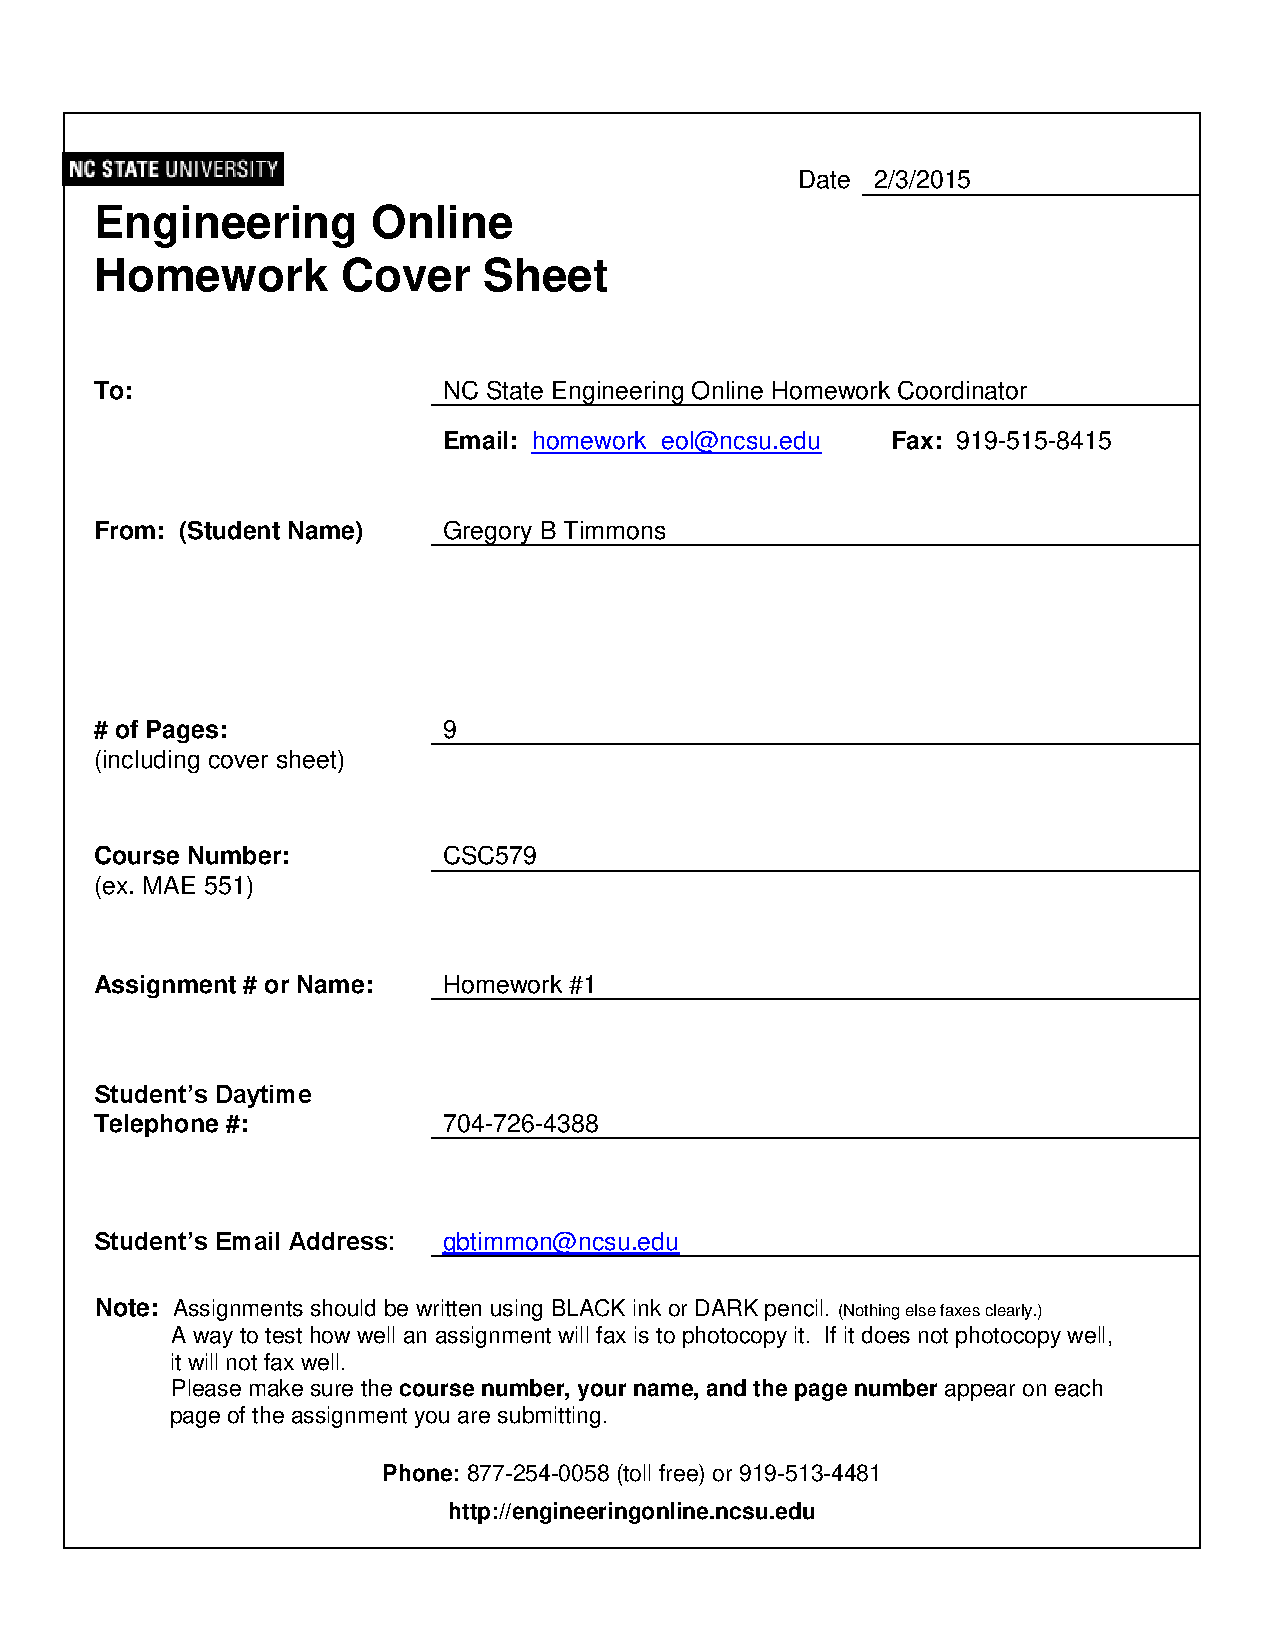
\includepdf[pages={1}]{cover.pdf}
\title{Homework 3}
\date{April 16, 2015}
\author{Gregory B Timmons, gbtimmon}
\maketitle

\section*{Question 1}	
\nn{ 
	\lambda 	&= 1,\\
	\alpha_1 	&= 0.5,\ \alpha_2 = 0.3,\ \alpha_3 = 0.2,\\
	\mu_1 		&= 4,\ \mu_2 = 2,\ \mu_3 = 1 
}

\begin{figure}[ht!]
\includegraphics[width=90mm]{STD_Question1.jpg}
\end{figure}
We have a QBD process and will compute Nuets R Matrix. 
\nn{\mm{
  	B_{00} & B_{01} & 0 & 0 & \ldots\\
  	B_{10} & A_1 & A_2 & 0  & \ldots\\ 
  	0      & A_0 & A_1 & A_2 & \ldots\\ 
  	0      & 0   & A_0 & A_1 & \ldots\\
 	\vdots&\vdots&\vdots&\vdots&\ddots 
 }}
 
\nn{
	B_{00} 	&= \mm{-\lambda}\quad \\
  	B_{01} 	&= \mm{\alpha_1\lambda & \alpha_2\lambda &\alpha_3\lambda}\\
  	B_{10} 	&= \mm{\mu_1\\\mu_2\\\mu_3} \\
	A_{0} 	&= \mm{
		\alpha_1\mu_1&\alpha_2\mu_1&\alpha_3\mu_1\\
		\alpha_1\mu_2&\alpha_2\mu_2&\alpha_3\mu_2\\
		\alpha_1\mu_3&\alpha_2\mu_3&\alpha_3\mu_3\\
	} \\
	A_{1} 	&= \mm{
		-(\mu_1 + \lambda) \\
		&-(\mu_2+\lambda)\\
		&&-(\mu_3 +\lambda)} \\
	A_{2} 	&= \mm{
		\lambda\\
		&\lambda\\
		&&\lambda
	}
}
Values : 
\nn { 
	A_{0} &= \mm{2&1.2&.8\\1& .6&.4\\.5& .3&.2}\\ 
   	A_{1} &= \mm{-6\\&-4\\&&-3} \\
   	A_{2} &= \mm{2\\&2\\&&2}     
}
V and W :
\nn{
	V &= A_2A_1^{-1} =\mm{-2/6\\&-2/4\\&&-2/3} \\
	W &= A_0A_1^{-1} =\mm{-1/3&-3/10&-4/15\\-1/6&-3/20&-4/30\\-1/12&-3/40&-4/60}
}
Now we compute Nuets R Matrix ( first 2 iterations) :
\nn{
	R_{(k+1)} &= -V - R^2_{(k)}\\
	R_0 &=\mm{0&0&0\\0&0&0\\0&0&0}\\
	R_1 &= -V -R_{(0)}^{2}W =\boxed{\mm{1/6\\&1/4\\&&1/3}}\\
	R_2 &= -V -R^2_{(1)}W = \mm{2/6\\&2/4\\&&2/3} - \mm{1/6\\&1/4\\&&1/3}^2
    \mm{-1/3&-3/10&-4/15\\-1/6&-3/20&-4/30\\-1/12&-3/40&-4/60}
    =\boxed{\mm{
	    .370  &  .033 &   .029 \\
	    .041 &   .537 &   .033 \\
	    .037 &   .033 &   .696
	 }}}
  
 \subsection*{Question 2}
\nn{
	 \mm{ \pi_0 & \pi_1 & \pi_2 & \pi_3 & \ldots }
	 \mm{
	  	B_{00} & B_{01} & 0 & 0 & \ldots\\
	  	B_{10} & A_1 & A_2 & 0  & \ldots\\ 
	  	0      & A_0 & A_1 & A_2 & \ldots\\ 
	  	0      & 0   & A_0 & A_1 & \ldots\\
	 	\vdots&\vdots&\vdots&\vdots&\ddots  
	 } = (0) 
}
This give us the following system of equations
\nn{
	\mm{\pi_0&\pi_1}\ \mm{
		 B_{00} & B_{01} \\ 
		 B_{10} & A_{1} + R * A_{0}
	}=\mm{0&0}
}
Or Explicitly 
\nn{
	\mm{\pi_{0} & \pi_{1_0} & \pi_{1_1} & \pi_{1_2}} 
 	\mm{-2&1&0.6&0.4\\ 4&-5&.6&.4\\2&1&-3.4&.4\\1&1&.6&-2.6} = \mm{0&0&0&0}
}
In order to get an exact solution we make the following small adjustments : 
 \nn{
 	\mm{\pi_{0} & \pi_{1_0} & \pi_{1_1} & \pi_{1_2}} 
 	\mm{-2&1&0.6&1\\ 4&-5&.6&0\\2&1&-3.4&0\\1&1&.6&0} = \mm{0&0&0&1}
 }
 
Which gives us
\nn{
    \pi   &= \mm{ 1&1&0.6&0} \\
    \pi_0 &= \mm{1}, \\
    \pi_1 &= \mm{1&0.6&0}
}

Next solve for $\alpha$ 
\nn{
    \alpha &= \pi_0 e  + \pi_1( I - R )^{-1}e = 24.59\\
    \pi_0 &= \mm{0.04066}\\
    \pi_1 &= \mm{0.04065 & 0.0243 & 0 }\\
    \pi_{(k+1)} &= \pi_{1}R^{k-1} 
}
 
Now we have the values to compute the values we are
looking for $\alpha$
\nn{
     p_0           &= ||\pi_{0}||_1 = \boxed{ 0.04066 } \\
     p_3           &= ||\pi_1R^2||_1 = \boxed { 0.03798 } \\
     p\{n \geq 4\} &= ||\pi_1R^{3}(I-R)^{-1}||_1 = 0.8094 \ \mbox{or}\\
      &=1 - p_0 - p_1 - p_2 - p_3 = 1 - ||\pi_{0}||_1 -
    ||\pi_{1}||_1 - ||\pi_{1}R||_1 - ||\pi_{1}||_1 =\boxed{0.8094}
 }
\subsection*{Question 3}
Arrival Time 
\nn{
	E[X] 	&= 16 \\
	Var(X) 	&= 32 \\
	C^2_X 	&= Var(X)/E[X]^2 = 1/8 
}
Departure Time
\nn{
	E[Y] 	&= \mu^{-1} = 12/60 
}
We need to build a distribution to model this arrival pattern.
\nn{
	r 		&= \lceil \frac{1}{(1/8)} \rceil\\
			&= \boxed{8}\\
	\alpha 	&=\frac{r - 2C_X^2 + \sqrt{r^2 + 4 -4rC_X^2}}{2(C_X^2 + 1)(r-1)}\\
			&=\frac{8 - 2C_X^2 + \sqrt{68 -32C_X^2}}{14C_X^2 + 14)} \\
			&=\frac{8 - 2(1/8)^2 + \sqrt{68 -32(1/8)^2}}{14(1/8)^2 + 14)} \\
			&= \boxed{1}\\
	\mu 	&= \frac{1 + 1(8-1)}{16}\\
			&= \boxed{1/2}
}
This suggests we can simulate this with a Erlang-8 distribution, $mu = .5$.\\
Checking the work:
\nn{
	E[X]	&= (1-\alpha)\frac{1}{\mu} + \alpha\frac{r}{\mu}\\
			&= (0) + \frac{8}{.5}\\
			&= 16\\
	Var[X] 	&= \frac{2(1-\alpha)+\alpha r(r+1)-(1-\alpha+\alpha r)^2}{\mu^2}\\
			&= \frac{2(1-1)+ 8(8+1)-(1-1+8)^2}{(.5)^2} \\
			&= \frac{72 - 64}{.25}\\
			&= 32
	}
The question can be modeled as a $E_r/M/1$ with $\lambda = 1/2, r = 8,$ and $
\mu = 1/12$ 
\nn{
	B_{00} &= \mm{
		-.5 & .5& 0 &\ldots\\
		0 & -.5& .5 &\ldots\\
		0 & 0& -.5 &\ldots\\	
		\vdots&\vdots&\vdots&	
	}\\
	B_{01} &= \mm{
		\vdots&\vdots&\vdots&\\
		0&0&0&\ldots\\
		0&0&0&\ldots\\
		.5&0&0&\ldots\\
	}\\
	B_{10} &=\mm{
		1/12 & 0 & 0 &\ldots\\
		0 & 1/12 & 0 &\ldots\\
		0 & 0& 1/12 &\ldots\\	
		\vdots&\vdots&\vdots&	
	}\\
	A_0 &= B_{10}\\
	A_2 &= B_{01}\\
	A_1 &= \mm{
		-(1/2+1/12) & .5& 0 &\ldots\\
		0 & -(1/2+1/12)& .5 &\ldots\\
		0 & 0& -(1/2+1/12) &\ldots\\	
		\vdots&\vdots&\vdots&	
	}
}

Using matlab code we compute the following attributes of this Ph/Ph/1 Queue. 
\nn{
	R &= \mm{
	  0 &       0 &       0 &      0  &      0  &      0  &      0  &      0\\
      0 &       0 &       0 &       0 &       0 &       0 &       0 &       0\\
      0 &       0 &       0 &       0 &       0 &       0 &       0 &       0\\
      0 &       0 &       0 &       0 &       0 &       0 &       0 &       0\\
      0 &       0 &       0 &       0 &       0 &       0 &       0 &       0\\
      0 &       0 &       0 &       0 &       0 &       0 &       0 &       0\\
      0 &       0 &       0 &       0 &       0 &       0 &       0 &       0\\
 0.9357 &  0.8755 &  0.8191 &  0.7664 &  0.7171 &  0.6710 &  0.6278 & 0.5874
  }\\
  \pi_0 &=\mm{0.0080 &  0.0156&   0.0226 &  0.0292 &  0.0354& 0.0411& 0.0465& 0.0516}\\
  \pi_1 &=\mm{0.0483& 0.0452& 0.0422& 0.0395& 0.0370& 0.0346& 0.0324 &0.0303 }
}

Now to compute the desired metrics: \\
\nn{
	p\{N_q \geq 2\} &= p\{N \geq 3\} \\
					&= || \pi_1 R^{2}(I-R)^{-1}||_1\\
					&= \boxed{0.2588}\\
	E[N] 			&= ||\pi_1(I-R)^-2||_1\\
					&= \boxed{1.8178}\\
	E[N_q]			&= E[N] - \lambda/\mu\\
					&= 1.8178 - 0.75\\
					&= 1.0678\\
	E[R]			&= E[R] = E[N]/\lambda \\
					&= \boxed{29.0848}
}
\end{document}